\chapter{Conceptos básicos}\label{preliminares}\label{basicos}

Este capítulo pretende ser una introducción a todos los conceptos teóricos necesarios para la correcta comprensión del trabajo que se detalla en esta memoria. 


\section{Procesamiento digital de imagen}\label{sec:procesamiento}
Un imagen $Q$ puede ser entendida como una función de dos variables, $q(x,y)$, donde $x$ e $y$ son las coordenadas en el plano de cada elemento (píxel) y la función da como resultado el nivel de gris o intensidad asociada a ese píxel. En concreto, cuando $x$ e $y$ así como la intensidad $q(x,y)$ son finitas y discretas hablaremos de que tenemos una imagen digital. Por eso mismo, el procesamiento digital de imagen se puede definir como aquel que se hace con imágenes digitales a través de un ordenador. Tiene su origen con la introducción de las primeras imágenes digitales a principios de 1920, donde se enviaban imágenes entre Londres y Nueva York por medio de un cable submarino.

Es claro que los seres humanos disponemos del sentido de la vista como el sentido más desarrollado para interacturar con el medio, pero esta está limitada a la banda visible dentro del espectro electromagnético. En cambio, el procesamiento digital de imagen puede cubrir el análisis de todo el espectro electromagnético, lo que incluye los ultrasonidos, el infrarrojos, rayos X, etc. Esta es la principal razón por la que el procesamiento digital de imagen puede incluirse en una gran cantidad de campos.\REV{quitar ultima frase?}

Dentro del procesamiento de imagenes digitales se encuentra la visión artificial. Esta es una subcampo de la inteligencia artificial (IA) y pretende emular la visión humana, incluyendo la capacidad de aprender así como el manejo directo de imágenes como datos de entrada a un problema dado. Actualmente, este campo está poco desarrollado \cite{lib:gonzalez} ya que el avance está siendo mucho más lento de lo que se esperaba en un primer momento. El análisis de imagen, que pretende entender cómo está formada la imagen, está situada a caballo entre la visión artificial y el procesamiento de imágen, y será lo que utilizaremos en este trabajo.

No hay una clara frontera entre el procesamiento de imagen y la visión artificial, esto hace que se hable de un paradigma que incluye 3 tipos de procesos; de bajo nivel, medio nivel y alto nivel. Dentro del nivel bajo se pueden incluir todos los procesos primitivos que tienen como objetivo reducir el ruido, realzar el contraste o ajustar la nitidez, por ejemplo. En un segundo nivel, más avanzado, se encuentran todos los procesos que tienen como entrada una imagen y obtienen atributos de esta. Pueden ser procesos como la segmentación (que se tratará aquí), descripción de objetos de la imagen o recocimiento de los mismos. En el último nivel se encuentran todas aquellas técnicas que hacen que todo ``tenga sentido'' ya que hacen que el análisis imite a la forma cognitiva de la mente humana.


\subsection{Imágenes digitales}\label{sec:imagenesdigitales}
Como ya se ha explicado en el apartado anterior, se habla de imagen digital cuando se puede ser capaz de determinar todos sus elementos (píxeles), es decir, estos son de forma finita y discreta. A partir de esta idea, se dispone de dos formas de representación para las imágenes en niveles de gris, en los rangos $[0,1]\in\RR$ y $[0,255]\in\NN$. En el primer caso diremos que la imagen está normalizada. Además, las imágenes digitales serán representadas por una matriz que contendrá cada uno de sus píxeles de manera ordenada.


\begin{figure}
\centering
    \subfigure[Niveles de gris]
    {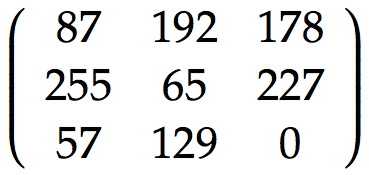
\includegraphics[height=0.1\textwidth]{img/matriznivelesgris.jpg}}\quad
    \subfigure[Normalizada]
    {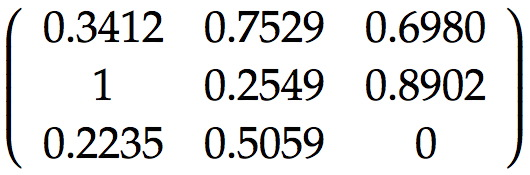
\includegraphics[height=0.1\textwidth]{img/matriznormalizada.jpg}}\quad\ 
    \subfigure[Gráfica]
    {
\includegraphics[width=0.1\textwidth]{img/imagendigital.jpg}}
    \caption{Imagen digital en diferentes representaciones.}
    \label{fig:defimagen}
\end{figure}

Como se puede apreciar en la figura \ref{fig:defimagen} cuanto más cercano a 0 sea el número, más negro será el nivel de gris, y cuanto más cercano a 1 ó 255, más blanco. En el caso de imágenes en color, se utiliza el formato RGB ({\em Red}, {\em Green} y {\em Blue}) donde existe una matriz como las anteriores por cada uno de los colores y al superponerlas se obtiene la imagen que vemos habitualmente.

\begin{definition}\label{def:histograma}
Se define el histograma de una imagen $Q$ con niveles de gris en el intervalo [0, 255] como la función $h(q) = n_q$ donde $n_q$ es el número de píxeles en la imagen con la intensidad $q$.
\end{definition}

Un ejemplo gráfico de la función de histograma para una imagen puede encontrarse en la figura \ref{img:rice}.


\subsection{Herramienta para el procesamiento digital: \MATLAB}\label{sec:matlab}
\MATLAB\ (abreviatura de {\em Matrix Laboratory}) es una herramienta de software matemático que ofrece un lenguaje de programación (lenguaje M) y un entorno de desarrollo integrado. Fue creado en 1984 por el informático y matemático Cleve Moler el cual buscaba una forma alternativa de ejecutar programas de álgebra en {\em Fortran}.

Entre sus prestaciones básicas están la manipulación de matrices, la representación de datos y funciones o la implementación de algoritmos así como la creación de interfaces de usuario (GUI). Además, el paquete básico de \MATLAB\ puede ser expandido por medio de {\em toolboxes}, como es el caso de este trabajo, donde se utilizará la relativa  a procesamiento de imagen. Se puede disponer también del software {\em Simulink} para trabajar conjuntamente a \MATLAB.

\subsection{Contraste}
Como en el trabajo se hace uso de imágenes con alto y bajo contraste, disponer una pequeña explicación. Pillar de los libros del laboratorio. \REV{Revisar}.

\subsection{Ruido en las imagenes}\label{sec:ruido}
Se condidera que una imagen está degradada cuando tiene ruido, esto es, cuando tiene defectos con respecto a la imagen original (fig. \ref{fig:defruido}). La principal fuente de ruido en images digitales se da en la adquisición o transmisión de las imagenes. Esto se puede deber a las condiciones ambientales o a la calidad de los sensores durante la toma de la imagen. Por ejemplo, la luminosidad, el polvo en el ambiente, etc. pueden ser determinantes. Por otra parte, en el caso de la transmisión, las imágenes pueden ser corrompidas por interferencias en el medio de transmisión, principalmente. Esto es claro cuando se transmite una imagen de un satélite, ya que la atmósfera interferir y provocar que la imagen recibida en la base terráquea no sea exactamente igual.
\begin{figure}
\centering
    \subfigure[Imagen original]
    {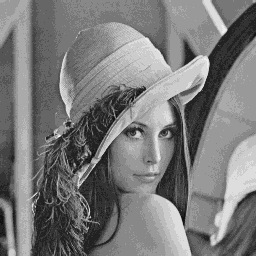
\includegraphics[width=0.3\textwidth]{img/lena}}\quad
    \subfigure[Imagen con ruido `sal y \mbox{pimienta}']
    {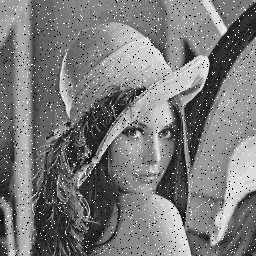
\includegraphics[width=0.3\textwidth]{img/lenas&p}}\quad
    \subfigure[Imagen con ruido gausiano]
    {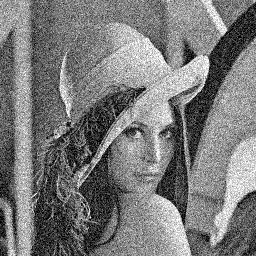
\includegraphics[width=0.3\textwidth]{img/lenaga}}
    \caption{Imagen de Lena con diferentes tipo de ruido}
    \label{fig:defruido}
\end{figure}

Las imágenes con ruido también se pueden crear artificialmente. Para ello utilizamos una cierta función $H$ de degradación, a la que añadimos un ruido al que llamaremos $\eta$ de forma que obtendremos una nueva imagen $g(x,y)$ que tendrá una serie de imperfecciones. Todo el ruido creado de esta forma se aplicará directamente sobre los píxeles de la imagen lo que provocará cambios en su histograma en una forma u otra. Aun así, debemos tener en cuenta que no hay relación directa entre la intensidad nueva que tienen los píxeles y la anterior. 

Existen muchos tipos de ruido como el exponencial, el gamma, el uniforme, etc. pero en esta memoria se han utilizado, el gausiano y el de tipo impulsivo o de `sal y pimienta'.

\subsubsection{Ruido gausiano}
Este puede ser uno de los modelos de ruido más utilizado en la práctica debido a que tiene una gran maleabilidad matemática. Basa su forma de actuar sobre la imagen en la función gausiana de probabilidad:
$$p(z) = \frac{1}{\sqrt{1}{2\pi\sigma}} e^\frac{-(z-\mu)^2}{2\sigma^2}$$
donde $z$ representa la intensidad, $\mu$ la media de $z$ y $\sigma$ la desviación estándar. Este tipo de ruido puede crearse en \MATLAB\ a través de la función \mintinline{matlab}{imnoise(img_var, 'gaussian')} sabiendo que \mintinline{matlab}{img_var} es la variable donde está almacenada la imagen en tipo \mintinline{matlab}{uint8}.

\subsubsection{Ruido de tipo `sal y pimienta'}
Este tipo de ruido, formalmente llamado impulsivo, hace que se conviertan píxeles de forma aleatoria en píxeles con intensidad 0 y 255. Esta es la razón de su particular nombre. De nuevo, fijándonos en \MATLAB, podremos crear imágenes con este tipo de ruido por medio del comando \mintinline{matlab}{imnoise(img_var, 'salt & pepper', prob_val)}, de nuevo \mintinline{matlab}{img_var} es la variable donde se almacena la imagen y \mintinline{matlab}{prob_val} es un valor entre 0 y 1 que hace las veces de probabilidad de la aparición del ruido. 

En este trabajo, se han utilizado imágenes con ruido para comprobar la adecuación o no de los algoritmos de segmentación al ruido. Ejemplos de ambos tipos de ruido se han presentado en la figura \ref{fig:defruido}.


% LOGICA DIFUSA
\section{Lógica difusa}\label{sec:logicadifusa}
La lógica difusa fue introducida por el matemático L. A. Zadeh \cite{art:zadeh} en 1965 con la intención de poder extender la lógica clásica o {\em crips} de forma que permitiera manejar y procesar la información que se compone de términos inexactos, imprecisos o subjetivos. Es, al fin y al cabo, un intento de imitar la forma de deducción del cerebro humano para trasladarlo a las máquinas. Se comenzará recordando la lógica clásica para después extender los conceptos a la difusa.

En primer lugar, definiremos el universo finito, $U$,  con el que se  trabajará, de forma que contenga todos aquellos elementos con los que se desee trabajar, esto es, $U = \{u_{1}, u_{2}, \dots, u_{n}\}$. En la lógica clásica simplemente asignamos verdadero o falso a cada uno de los elementos del conjunto que se estudia. Por esta razón, al definir un conjunto $A$ podremos decir que este contiene o no a los elementos del universo $U$ con una certeza absoluta. De esta manera, daremos un valor de 1 cuando $u_{i}$ esté incluido en $A$ (verdadero) y un valor de 0 cuando no lo esté (falso). En esta última idea se refleja por medio de la función de pertenencia al conjunto  $A$, $\mu_{A}$ (ecuación \ref{eq:logicaclasica}).
\begin{equation}\label{eq:logicaclasica}
\begin{aligned} 
	A = \{(u_{i}, \mu_{A}(u_{i})) | u_{i}\in U\}\\
	\mu_{A}:U\rightarrow \{0,1\} \text{ tal que}\\
	\mu_{A}(u) = \left\{ \begin{aligned}
		1 \quad\text{si}\quad u\in A\\
		0 \quad\text{si}\quad u\notin A
 	\end{aligned}\right.
\end{aligned}
\end{equation}
%\REV{revisar ecuación con respecto al ejemplo} Se da más adelante la concreta.

 Podemos considerar el problema de determinar si una persona es alta o no. Para la lógica clásica, este razonamiento se simplificará en buscar un valor a partir del cual podamos definir que cierta persona es alta. Para el siguiente ejemplo, tomaremos 1,75 metros como referencia, donde $A$ es el conjunto de las personas altas. De este modo, $\mu_{A}=1 \text{ si } u>1,75$ y en otro caso $\mu_{A}=0$. En la figura \ref{fig:altoclasica} se puede ver la representación del concepto `alto' para las posibles alturas que se pueden presentar.

\subfile{graficos/logicaclasicagraf}

Por otra parte, la lógica difusa dispone de la función de pertenencia más compleja, lo que nos hace poder decir que alguien es `poco alto' o `bastante alto' ya que no daremos un par de valores ($\{0,1\}$) sino cualquiera de los contenidos en el intervalo que definen. Así $\mu_{A}$ será una función que asigna un valor entre 0 y 1 a cada elemento de $A$.\begin{equation}\label{eq:logicadifusa}
\begin{aligned} 
	A = \{(u_{i}, \mu_{A}(u_{i})) | u_{i}\in U\}\\
	\mu_{A}:U\rightarrow [0,1]
\end{aligned}
\end{equation}                
Si continuamos con el ejemplo se verá que el conjunto alto ($A$) esta vez se define como explica la ecuación \ref{eq:ejemplodifusa}. 

\begin{equation}\label{eq:ejemplodifusa}                
	\mu_{A}(u) = \left\{ \begin{aligned}
		1 \quad&\text{si}\quad u\geq 2\\
		2u - 3 \quad&\text{si}\quad 1.5>u>2\\
		0 \quad&\text{si}\quad u\leq 1.5
 	\end{aligned}\right.
 \end{equation}           
Esta nueva función de pertenencia hace que podamos distinguir 3 zonas dentro de su representación (figura \ref{fig:altodifusa}). Se tendrá de nuevo la etiqueta `alto' y `no alto' que hacen que su pertenencia sea certera. Se dispondrá, también, una parte de la pertenencia a la que llamaremos `difuso' donde el conjunto no afirma ser ni `alto' ni `no alto' sino que está en una situación intermedia. En este caso se habla de que el elemento $a_{i}$ que se encuentra ahí pertenece a $A$ con grado $\mu_{A}(a_{i})$.
                
\subfile{graficos/logicadifusagraf}

Más formalmente, denotaremos al conjunto que incluye a todos los conjuntos difusos como $\FF(u)$ a todos aquellos que se encuentran definidos sobre un referencial finito ($|U| = n$) por lo que $U$ no será un conjunto vacío.
 


% FUNCIONES REF
\section{Funciones de equivalencia restringida (REF)}\label{sec:ref}
El concepto de función de equivalencia restringida (REF por sus siglas en inglés) surge del concepto de equivalencia y el de similitud \cite{art:refbarrenechea}. Este concepto es muy utilizado para la comparación de imágenes y su intención es dar una medida de cómo de iguales o similares son dos elementos $x$ e $y$. Para poder definir el concepto de REF, necesitamos varios previamente. 

\begin{definition}\label{def:negacionestricta}
Una negación estricta es aquella función $c : [0, 1] \rightarrow [0, 1]$ que cumple que $c(0)=1$ y $c(1)=0$ y es estrictamente decreciente y continua. Además, si $c$ es involutiva se considera que se habla de una negación fuerte.
\end{definition}

\begin{definition}\label{def:automorfismo}
Llamaremos automorfismo ($\varphi$) a todas aquellas funciones del intervalo unidad tal que $\varphi : [0, 1] \rightarrow [0, 1]$ sean continuas y estrictamente crecientes propiciando que $\varphi(0)=0$ y $\varphi(1)=1$.
\end{definition}

En 1979, E. Trillas \cite{art:thtrillas} enunció el siguiente teorema. 
\begin{theorem}[Teorema de Trillas]\label{th:trillas}
Una función $c : [0, 1] \rightarrow [0, 1]$ es una negación fuerte si, y sólo si, existe un automorfismo del intervalo unidad tal que $c(x)=\varphi^{-1}(1-\varphi(x))$.
\end{theorem}

\begin{definition}\label{def:ref}
Una función $REF  : [0, 1] \rightarrow [0, 1]$ es llamada de equivalencia restringida cuando cumple que:
	\begin{enumerate}
	\item $REF(x, y) = REF(y, x), \forall x, y \in [0, 1];$
	\item $REF(x, y) = 1$, si y sólo si, $x=y$;
	\item $REF(x, y) = 0$, si y sólo si, $x=1$ e $y=0$ ó si $x=0$ e $y=1$;
	\item $REF(x, y) = REF(c(x), c(y)),  \forall x, y \in [0, 1]$, siendo $c$ una negación fuerte.
	\item $\forall x, y, z \in [0, 1]$, si $x\leq y\leq z$, entonces $REF(x, y)\geq REF(x, z)$ y  $REF(y, z)\leq REF(x, z)$
	\end{enumerate}
\end{definition}

\begin{proposition}\label{prop:contruccionref}
Sean dos automorfismos $\varphi_{1}$ y $\varphi_{2}$, se llamará función $REF$ a la construcción que cumpla que: 
$$REF(x,y) = \varphi_1^{-1}(1-|\varphi_2(x)-\varphi_2(y)|) \quad\text{con}\quad c(x) = \varphi_2^{-1}(1-\varphi_2(x)).$$ 
Además, si tenemos una $REF$ y un automorfismo en $\unitinterval$, la aplicación de estos ($F=\varphi \circ REF$) es otra $REF$.
\end{proposition}

\begin{theorem}\label{th:ref}
Una función continua $REF:\unitinterval^2 \rightarrow\unitinterval$ que cumpla que $REF(1,x)=x, \xinunitinterval$, es una función $REF$ asociada con la función $I:\unitinterval^2\rightarrow\unitinterval$ con $I$ continua y asociativa si y sólo si existe un automorfismo $\varphi$ en $\unitinterval$ tal que:
$$REF(x,y)=\varphi^{-1}(1-\abs{(\varphi(x)-\varphi(y))})\quad\text{ y }\quad c(x)=\varphi^{-1}(1-\varphi(x))$$
\end{theorem}

%\REV{Teorema que hace que estos automorfismos puedan ser 1 solo?} No lo pongo pq no lo utilizo.


% FUNCIONES DE AGREGACIÓN
\section{Funciones de agregación}\label{sec:agregacion}
%\REV{funciones de agregación vs operadores de agregación ¿Qué es más correco para nombrarlos?} -> Funciones de agregación.
Las funciones de agregación tienen como propósito reducir las dimensiones de la información a partir de la combinación de los datos de entrada obteniendo una salida que los represente \cite{art:montero, art:calvoagregacion}. Su aplicación se extiende en muchos casos prácticos y teóricos como la lógica multievaluada, control difuso, la toma de decisión, etc \cite{art:paternain}.  Se definirá una función de agregación como sigue:

\begin{definition}\label{def:agregacion}
Se dice que $M : \unitinterval^n \rightarrow \unitinterval$ es una función de agregación de dimensión $n$ siempre que satisfaga:
	\begin{enumerate}
	\item $M(x_1, \dots, x_n) = 0$ si y sólo si $x_1=\dots=x_n=0$;
	\item $M(x_1, \dots, x_n) = 1$ si y sólo si $x_1=\dots=x_n=1$;
	\item $M$ es una función estrictamente creciente.
	\end{enumerate}
\end{definition}
\begin{definition}
Una función de agregación $M$ será llamada media si
$$ \min(x_{1}, \dots, x_{n})  \leq M(x_{1}, \dots, x_{n}) \leq \max(x_{1}, \dots, x_{n}).$$
\end{definition}

En este proyecto se utilizarán mayoritariamente las funciones de agregación idempotentes, esto es, que cumplen que $M(x,\dots ,x)=x, \forall x$. En particular, una función de agregación idempotente es una media. Entre las funciones que utilizaremos encontramos la media aritmética, el mínimo, el máximo o la media geométrica. Además, se definen a continuación otras que no son de uso tan común.
% OWA
\subsection{Funciones OWA}
En esta sección se introduce el concepto de las funciones de media ponderada ordenada (OWA, {\em  ordered weighted averaging}) \cite{art:yagerowa, art:paternain, art:bustinceowa}. Se basan en la idea de generar una media, ordenando primero los elementos a agregar, para luego darles mayor relevancia a una parte de ellos. Este tipo de función generaliza la media aritmética, siendo esta el OWA en el que todos los elementos del vector de pesos son iguales.

\begin{definition}\label{def:owa}
Una  función $F:\unitinterval^n\rightarrow\unitinterval$ será una función OWA de dimensión $n$ si existe un vector $w=(w_{1},w_{2},\dots,w_{n})\in \unitinterval^{n}$ tal que $\sum_{i}w_{i}=1$ de forma que
$$F(x_{1},\dots,x_{n})=\sum^{n}_{j=1}w_{j}x_{\sigma(j)}$$
donde $x_{\sigma(j)}$ es el $j$-ésimo mayor elemento del vector $(x_{1},\dots,x_{n})$.
\end{definition}

Por tanto para poder obtener un resultado adecuado, deberá utilizarse un vector de pesos $w$ que se adecúe a las necesidades del problema. En este trabajo se emplea la versión `al menos la mitad' %\REV{nombre}. Solucionado.
 que tiene como vector de pesos aquel que se obtiene con la ecuación \ref{eq:pesosowamayoria}. Esto generará una agregación donde destaquen todos aquellos elementos que se encuentren por detras de la mediana.
% a $w=(w_{1}\dots w_{i}, w_{i+1}\dots w_{n})$ sabiendo que $\abs{1, \dots, i}=\abs{i+1,\dots,n}$ de forma que $w_{j}=\frac{1}{2n}$ si $1\leq j\leq i$ y $w_{j}=0$ en el resto de los casos.\REV{buscar la versión buena, esto es sólo para los cardinales pares}.\REV{volver a redactar. Incluir construcción.}

\begin{equation}\label{eq:pesosowamayoria}
	 w_i = Q\left(\frac{i}{t+1}\right) - Q\left(\frac{i+1}{t+1}\right), \forall i\in \{1, \dots, n\}, \text{   sabiendo que}
\end{equation}
	 $$Q(r) = \left\{\begin{aligned}
	 	0 					&\quad \text{si}\quad r<0,5\\
	 	\frac{r-0,5}{0,5}	&\quad \text{si}\quad 0,5\leq r\leq 1\\
	 	1 					&\quad \text{si}\quad r>1\\
	\end{aligned}\right.$$
%\REV{forma ecuación}

%\REV{reescrito}
Además, en la segunda parte del estudio, se emplea el OWA `la mayoría de'. Este OWA pretende destacar aquellos elementos que son mayores en el vector $x$. Esto se hace realidad por medio de un vector de pesos donde son nulos los pesos relativos a aquellas $x_i$ más pequeñas. Para la construcción del vector de pesos, se utilizará, también, la ecuación \ref{eq:pesosowamayoria}



% CHOQUET
\subsection{Integral Choquet}
Para este otro tipo de función \cite{art:choquet, art:sugenochoquet} de agregación se pretende dar una nueva de forma de representar un conjunto de datos en una única salida. De esta forma, se define primeramente una medida a través de la cual se calculará la forma en la que cada elemento del conjunto de datos tendrá reelevancia en la agregación final. Para ello definimos el concepto de medida difusa.
\begin{definition}\label{def:medidadifusa}
Dado $U$ un universo finito; $\mathcal{P}(U)$ el conjunto de todos los subcojuntos de $U$. Una medida difusa es una función $\mu:\mathcal{P}(U)\rightarrow\unitinterval$ que satisface que:
\begin{enumerate}
	\item $\mu(\emptyset)=0$ y $\mu(U)=1$.
	\item $A\subseteq B \Rightarrow \mu(A)\leq\mu (B), \forall A, B \subseteq U$.
\end{enumerate}
\end{definition}

A continuación definimos la función integral Choquet conociendo que tomaremos su versión discreta por el contexto en el que se está trabajando.

\begin{definition}\label{def:choquet}
Dado un vector $(x_1,\dots,x_n)$, sea $\sigma$ una permutación de $\{1,...,n\}$ tal que $x_{\sigma(j)}$ es el $j$-ésimo mayor elemento del vector $(x_{1},\dots,x_{n})$. La integral discreta de Choquet con respecto a la medida difusa $\mu$ es 
$$Ch_{\mu}(x)=\sum_{i=1}^{n}x_{\sigma(i)}(\mu(\{\sigma(i),\dots,\sigma(n)\})-\mu(\{\sigma(i+1),\dots,\sigma(n)\}))$$
tomando la convención de que $\{\sigma(n+1),\sigma(n)\}=\emptyset$.
\end{definition}

\begin{proposition}\label{prop:choque2owa}
Si denotamos a $w_{\sigma, i}^{\mu} = \mu(\{\sigma(i),\dots,\sigma(n)\})-\mu(\{\sigma(i+1),\dots,\sigma(n)\})$ se obtiene la siguiente definición de la integral Choquet en función de los operadores OWA definidos en \ref{def:owa}:
$$\sum_{i=1}^{n} w_{\sigma, i}^{\mu} \cdot x_{\sigma(i)}.$$
\end{proposition}


% FUNCIONES DE SIMILITUD
\section{Funciones de similitud}\label{sec:similitud}
El concepto de similitud \cite{art:fan1, art:fan2} surge cuando queremos medir cómo de parecidos son dos conjuntos difusos. Este concepto es muy parecido al de REF, pero en este caso se consideran conjuntos y no elementos. Por esta razón, utilizamos las REF como base para definir las funciones de similitud.
\begin{definition}\label{def:similitud}
Dada una función $M$ de agregación (definición \ref{def:agregacion}) y una función $REF$ (definión \ref{def:ref}) llamaremos a $SM$ función de similitud si $SM : \FF(X) \times \FF(X) \rightarrow [0,1]$ está definida tal que 
$$SM(A,B)=M^n_{i=1}REF(\mu_A(x_i), \mu_B(x_i))$$
y satisface las siguientes condiciones:
	\begin{enumerate}
	\item $SM(A, B) = SM(B, A), \forall A, B \in \FF(X)$;
	\item $SM(A, A_c) = 0$, si y sólo si A no es difuso;
	\item $SM(A, B) = 1$ si y sólo si A = B;
	\item Si $A\leq B\leq C$, entonces $SM(A, B)\geq SM(A,C)$ y $SM(C, B)\geq SM(C,A)$;
	\item $SM(A_c, B_c) = SM(A,B)$
	\end{enumerate}	
\end{definition}

\begin{remark}\label{obs:funcionesref}
Durante el desarrollo de este trabajo se buscará la similitud entre conjuntos difusos y el conjunto $\tilda1$. Se define el conjunto $\tilda1 =\{(u_{i}, \mu_{\tilda1}(x)=1)|u_{i}\in U \}$, esto es, aquel en el que todos sus elementos tienen pertenencia absoluta.
\end{remark}


% FUNCIONES PENALTI
\section{Funciones penalti}\label{sec:penalti}
Una función penalti  \cite{art:calvo} es una función de agregación, por lo que dispone de un vector de entradas del que devuelve un único resultado. Si todos los elementos del vector son iguales, entonces, claramente, la salida será eso mismo. Ahora bien, el problema surge cuando hay algún elemento diferente ya que en ese momento la idea será buscar una salida todo lo parecida posible a la entrada. En este sentido, es elemento o elementos diferentes tendrán una cierta discrepancia con los demás y justamente esto es lo que se pretende minimizar, la discrepancia, para dar una salida adecuada. 

\begin{definition}\label{def:penalti}
La función $P:[a,b]^{n+1}\rightarrow \RR^{+} = [0, \infty]$ es una función penalti si y sólo si satiface que:
\begin{enumerate}
	\item $P(x, y) \geq 0, \forall x, y$
	\item $P(x, y) = 0$ si $x_{i}=y \forall i=1,\dots ,n$
	\item $P(x,y)$ es cuasiconvexa en $y$ para cualquier $x$, esto es, $P(x, \lambda\cdot y_{1} +(1-\lambda)\cdot y_{2})\leq \max(P(x, y_{1}), P(x, y_{2}))$.
\end{enumerate}
\end{definition}
La función en la que se basan las penalti es $$f(x)=\arg\min_{y} P(x,y)$$ si $y$ es el único mínimo e $y=\frac{a+b}{2}$ si el conjunto de minimizadores es el intervalo $(a, b)$.

\begin{theorem}
Todas las funciones de agregación llamadas medias pueden ser escritas como una función basada en una función penalti expresada en la definición \ref{def:penalti}.
\end{theorem}


% FUNCIONES DE DOMBI
\section{Funciones de Dombi}\label{sec:dombi}
Las funciones de Dombi \cite{art:dombi} son operadores de equivalencia con una definición diferente a las REF presentadas en la sección \ref{sec:ref}. Con esta relación lo que se pretende conocer es como de iguales son dos elementos de un conjunto difuso dado, pero aplicando nuevas ideas para la construcción del resultado. 
%\REV{Definición completa?} Pues así se va a quedar.
\begin{definition}\label{def:dombi}
Dados $x=(x_1, x_2, \dots,x_n)$ y $w=(w_1,w_2,\dots,w_n)$, denotaremos $D$ como una función de equivalencia de Dombi cuando tengamos que 
$$D(w,x)=\frac{1}{2}\left(1+\prod(1-2x_{i})^{w_{i}}\right)$$
\end{definition}
\begin{lemma}\label{def:propiedadesdombi}
La función de equivalencia de Dombi, $D$, cumple las siguientes propiedades:
\begin{enumerate}
	\item $D:\unitinterval\times\unitspace \text{ es continua}$;
	\item $D((w_1,w_2),(0,0)) = 1$;\quad$D((w_1,w_2),(1,1)) = 1$;
	\item $D((w_1,w_2),(0,1)) = 0$;\quad$D((w_1,w_2),(1,0)) = 0$;
	\item $D((w_1,w_2),(x,c(x))) = 0$.
\end{enumerate}
\end{lemma}
%\REV{propiedades}



%NOTACIÓN
\section{Notación}\label{sec:notacion}

A lo largo del trabajo se asumirá la notación que sigue para estos conceptos.

\begin{description}
    \item[Imagen]: la denotaremos con $Q$.
    \item[Coordenadas de un pixel]: $(x,y)$.
    \item[Máximo nivel de gris]: $L$.
    \item[Número de filas de $Q$]: $N$.
    \item[Número de columnas de $Q$]: $M$.
    \item[Intensidad de un pixel]: $q(x,y)$ de forma que $0\leq q(x,y)\leq L-1, \forall (x,y)\in Q$.  
    \item[Histograma]: $h(q)$. Función para conocer el número de pixeles con la intensidad $q$. 
    \item[Media de una imagen]:$$m_Q=\frac{\sum_{q=0}^{L-1}qh(q)}{\sum_{q=0}^{L-1}h(q)}$$
    \item[Área de una imagen]: $$A(Q) = \sum_{q=0}^{L-1} q h(q)$$
\end{description}

